\section{The Value Problem in Wind Energy}\label{sec:value_problem}

Supply-side indicators such as installed capacity in gigawatts or annual generation in terawatt-hours are commonly used to measure the growth of wind energy. However, these metrics overlook a key economic tension: as more wind power enters the system, the wholesale market value of each additional unit of generation tends to decline. For investors and policymakers, this directly shapes whether an offshore wind project remains financially viable. This section examines the mechanisms behind that value erosion, focusing on the merit order effect, domestic and cross-border cannibalisation, and the way revenue support instruments interact with these dynamics.

\subsection{Market Value and the Value Factor}\label{sec:market_value}

On European wholesale electricity markets, generators are paid based on the price at the hour they produce. A baseload plant running around the clock earns approximately the time-averaged wholesale price. A wind farm, by contrast, earns a price determined by the hours when it generates. Because wind output concentrates during specific meteorological conditions that tend to coincide across a region's fleet, this generation-weighted average price can differ substantially from the baseload average.

\begin{figure}[ht]
    \centering
    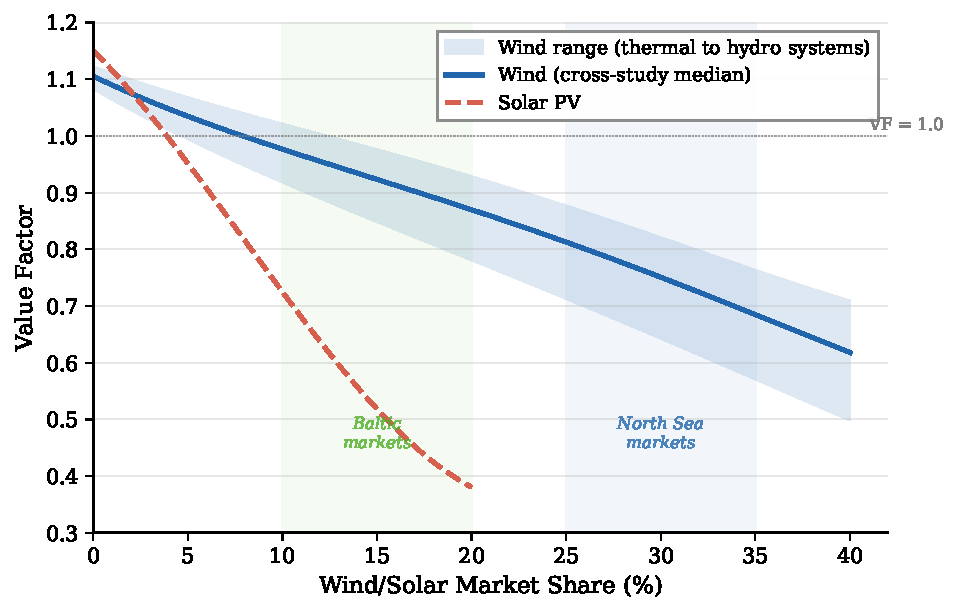
\includegraphics[width=0.68\textwidth]{value_factor_decline.pdf}
    \caption{Value factor decline with increasing wind and solar market share, synthesised from empirical data and modelling results in Hirth \cite{Hirth2013}. The shaded band for wind reflects the range between thermal-dominated systems (lower bound) and hydro-dominated systems (upper bound). Approximate current penetration ranges for North Sea and Baltic markets are indicated.}
    \label{fig:value_factor_decline}
\end{figure}

\vspace{4pt}

Two metrics have become standard for quantifying this erosion, both formalised by Hirth \cite{Hirth2013}. The \textit{capture price} is the generation-weighted average spot price that a wind farm receives over a given period. The \textit{value factor} is the ratio of the capture price to the baseload price:
%
\begin{equation}
    \text{Value Factor} = \frac{\text{Capture Price}}{\text{Baseload Price}} = \frac{\sum_{t} p_t \cdot g_t}{\bar{p} \cdot \sum_{t} g_t}
    \label{eq:value_factor}
\end{equation}
%
where $p_t$ is the spot price and $g_t$ is the wind generation at hour $t$, and $\bar{p}$ is the time-averaged baseload price. At low penetration levels, value factors sit near or above unity; as wind's share of the electricity mix grows, the value factor declines because wind output is large enough to move wholesale prices during the hours it generates.

\vspace{4pt}

Hirth's \cite{Hirth2013} early estimates, drawing on data through 2012, placed the value factor decline at approximately 1.10 at negligible penetration to between 0.50 and 0.80 at a 30\% wind share (Figure~\ref{fig:value_factor_decline}), with the range reflecting differences between thermal-dominated systems (lower bound) and hydro-dominated systems (upper bound). Subsequent empirical work covering higher penetration levels has confirmed and sharpened this pattern \cite{Stiewe2025, LopezProl2024, Ember2025, BalticCannibalisation2024}, while revealing that the decline accelerates at the penetration levels North Sea markets now occupy. The distinction between thermal and hydro systems is directly relevant to the North Sea--Baltic comparison: most North Sea markets are thermal-heavy, while the Baltic benefits from Scandinavian hydropower. Yet no existing study has systematically measured and compared value factors across the full set of bidding zones surrounding both basins.

\begin{figure}[ht]
    \centering
    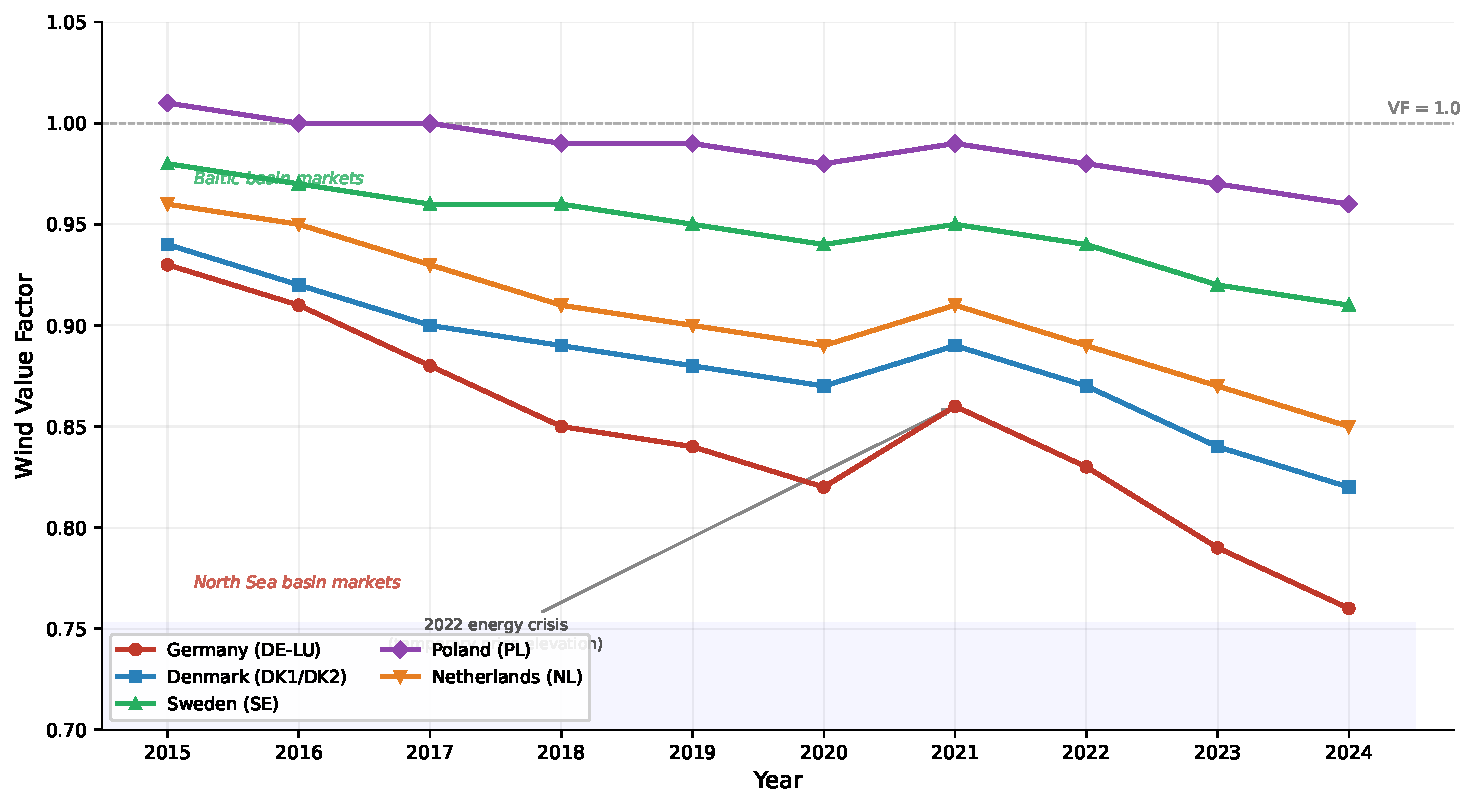
\includegraphics[width=0.8\textwidth]{value_factor_trajectories.pdf}
    \caption{Empirical wind value factor trajectories for selected European bidding zones, 2015--2024. Value factors are computed as the ratio of the generation-weighted capture price to the baseload average price. Data synthesised from Stiewe et al. \cite{Stiewe2025}, Ember \cite{Ember2025, EmberGlobal2024}, and ACER market monitoring reports \cite{ACER2023, ACER2025}. The 2021--2022 uptick reflects the temporary elevation of wholesale prices during the European energy crisis.}
    \label{fig:vf_trajectories}
\end{figure}


\vspace{4pt}

Figure~\ref{fig:vf_trajectories} confirms this pattern empirically, tracking the wind value factor across five European bidding zones from 2015 to 2024. The divergence between basins is clear: Germany's value factor fell from 0.93 to 0.76 as wind penetration rose from roughly 20\% to 35\%, while Poland, where wind remained below 18\% of generation and coal sets the marginal price for most hours, stayed near unity. The Scandinavian markets occupy an intermediate position, buffered by flexible hydropower. A brief upward correction is visible in 2021 and 2022 when the gas price crisis elevated wholesale prices faster than capture prices could follow; once gas markets normalised, the structural decline resumed. The spread between the highest and lowest trajectories widened from five percentage points in 2015 to twenty by 2024, demonstrating both the severity of value erosion and the necessity of basin-level comparison.


\subsection{The Merit Order Effect}\label{sec:merit_order}

European day-ahead electricity markets operate under pay-as-clear pricing. Generators bid their short-run marginal cost, and the market operator clears demand against an ascending supply curve, or merit order, paying all dispatched units the price set by the most expensive unit needed to meet demand. Wind turbines, with near-zero marginal cost, enter at the bottom of this curve. As wind output increases, the supply curve shifts rightward, displacing higher-cost thermal generators and reducing the clearing price. This is the merit order effect. Figure~\ref{fig:merit_order} illustrates this mechanism schematically.

\begin{figure}[ht]
    \centering
    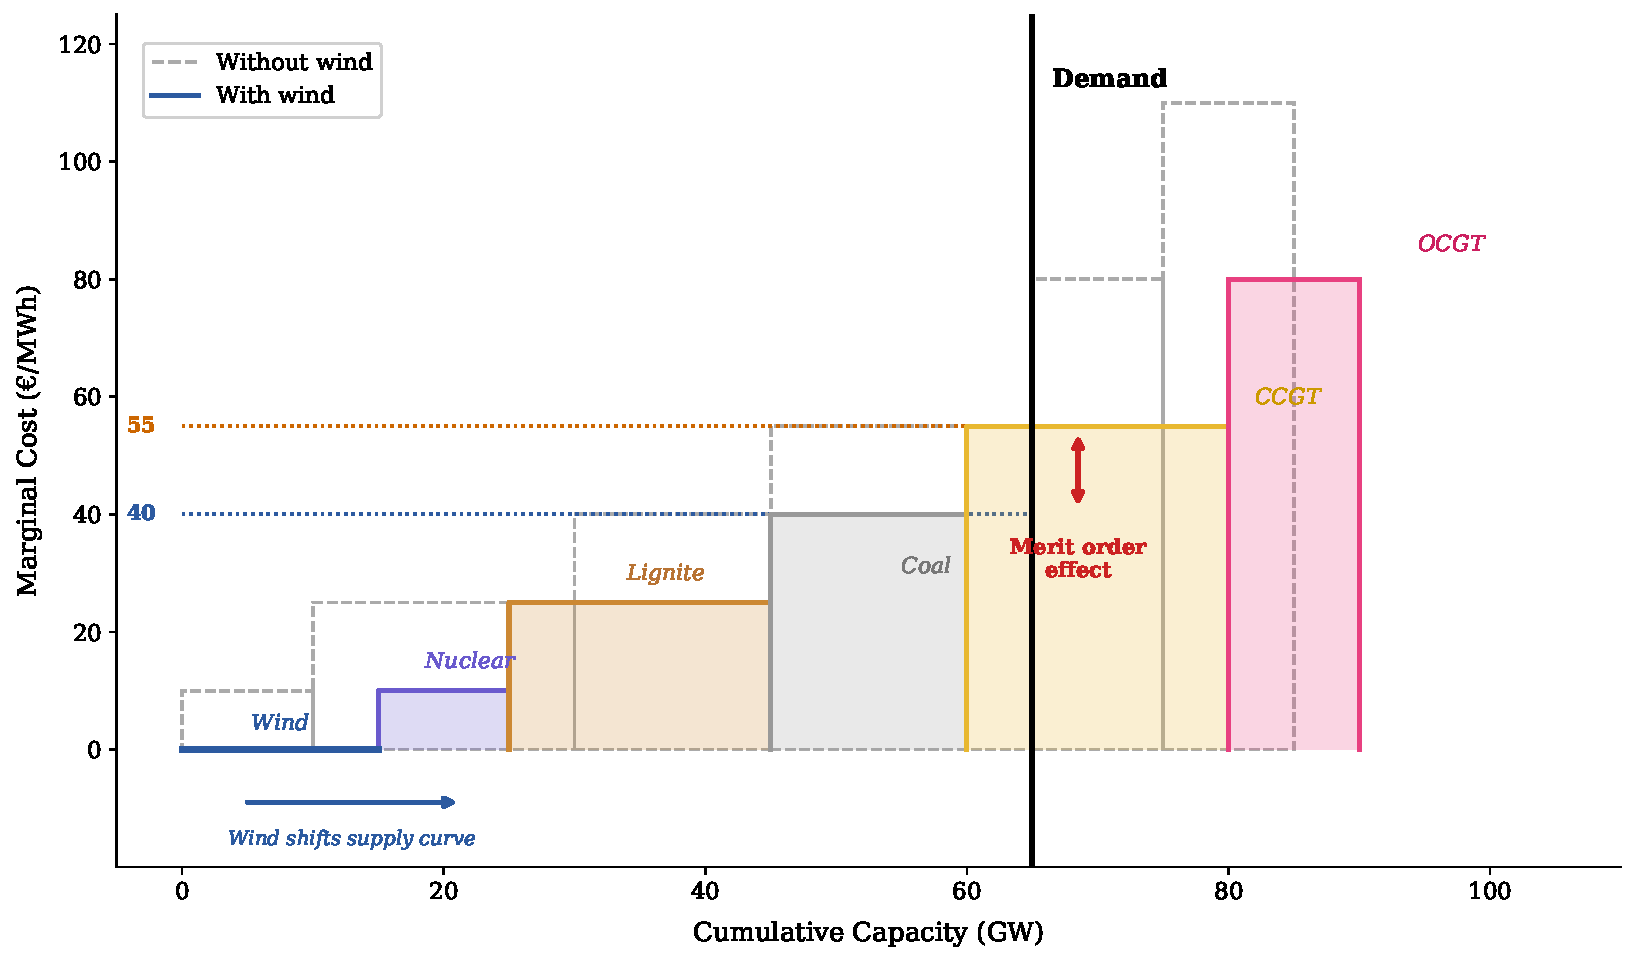
\includegraphics[width=0.8\textwidth]{merit_order_effect.pdf}
    \caption{Schematic illustration of the merit order effect. When wind generation enters at the bottom of the supply curve, it shifts the curve to the right, displacing higher-cost thermal generators and reducing the market clearing price from 55 to 40~\euro/MWh in this stylised example. The price depression is greatest during hours of high wind output.}
    \label{fig:merit_order}
\end{figure}

Country-specific MOE estimates span a wide range, from the foundational 7.83~\euro/MWh estimated by Sensfu\ss{} et al. \cite{Sensfuss2008} for Germany in 2006 using agent-based simulation, through to 13~\euro/MWh in Cludius et al.'s \cite{Cludius2014} later econometric analysis of the same market, and down to 0.4~\euro/MWh in the Czech Republic (0.04~ct/kWh, \cite{Lunackova2017}). This more-than-an-order-of-magnitude dispersion reflects not only genuine differences in market structure and time period but also methodological fragility: agent-based simulations depend on assumptions about bidding behaviour that are difficult to validate \cite{Sensfuss2008}, while econometric approaches struggle to separate the wind-induced price effect from correlated demand and fuel price movements \cite{Wurzburg2013, Clo2015, Kolb2020}. Published MOE estimates for Baltic markets are entirely absent from the literature, with the pan-European study by Cevik and Ninomiya \cite{Cevik2022} providing the only estimates that encompass Baltic bidding zones. This absence is itself a finding: the merit order effect in Baltic electricity markets remains unquantified.

\vspace{4pt}

The most comprehensive cross-country estimate comes from Cevik and Ninomiya \cite{Cevik2022}, whose panel quantile regression across 12 European countries over 2014--2021 finds that each percentage point increase in renewable electricity share reduces average wholesale prices by 0.6\%, with the effect accelerating nonlinearly at higher penetration levels. This nonlinearity, combined with the fact that wind generators sell electricity precisely during the hours when prices are most depressed by their own collective output \cite{Hirth2013}, explains the severity of value erosion in markets that have already exceeded the welfare-optimal wind share of approximately 20\% estimated by Hirth \cite{HirthOptimal2015}. That said, their country-level annual aggregation may mask the within-day dynamics most relevant to capture value computation, and their sample excludes several Baltic markets where the MOE is most poorly understood.

\vspace{4pt}

Offshore wind exhibits a particularly pronounced merit order effect compared to onshore wind: higher and more consistent capacity factors produce output that is more temporally concentrated and spatially correlated across assets in the same sea basin, so that sustained periods of strong wind across the North Sea depress clearing prices simultaneously across multiple interconnected bidding zones \cite{Yamujala2026}.

\subsection{Cannibalisation: Domestic and Cross-Border}\label{sec:cannibalisation}

\subsubsection{Domestic cannibalisation}

While the merit order effect describes price suppression at a given moment, cannibalisation captures its cumulative, structural consequence: as more wind capacity enters a market over months and years, it reduces the revenue earned per megawatt-hour by all existing and new wind assets. Its severity depends on the interaction between VRE penetration, the spatial correlation of wind output, fuel and carbon prices, and the flexibility of the broader power system \cite{Hirth2013, Stiewe2025}. The regional variation in these factors across the North Sea and Baltic is examined in Section~\ref{sec:regional_drivers}; here, the focus is on the mechanisms and their empirical magnitude.

\vspace{4pt}

The most visible symptom is the growing incidence of negative wholesale electricity prices. When abundant wind generation coincides with inflexible baseload plants (nuclear, lignite, combined heat and power) that refuse to curtail, and wind generators continue producing under out-of-market support incentives, the clearing price is pushed below zero. Negative price hours across European markets have risen substantially, concentrated in zones with the highest wind and solar penetration \cite{Ember2025, EmberGlobal2024}. The 2022 energy crisis temporarily masked this trend by elevating wholesale prices, but as gas prices normalised, the structural pattern reasserted itself with greater severity \cite{Ruhnau2023}.

\vspace{4pt}

Germany's experience quantifies the acceleration of domestic cannibalisation. The wind value factor declined from 0.93 in the early 2010s to 0.76 by 2024 as penetration rose from roughly 20\% to 35\%, driven by the compounding effects of higher penetration, increased temporal concentration of offshore wind output, and the structural inflexibility of lignite-based baseload capacity \cite{Monteil2023, Stiewe2025, Ember2025}.

Whether cannibalisation is permanent or transient depends on the interplay between market structure and policy design. Theoretical models suggest convergence under idealised conditions \cite{Antweiler2021, Brown2021}, but current European markets combine carbon pricing with direct VRE support mechanisms that decouple investment decisions from market signals \cite{Hirth2013}, delaying or preventing the equilibrating exit of marginal generators that these models rely on. The gap between theory and practice is particularly stark in small, rapidly expanding Baltic markets. A 2024 study of renewable expansion scenarios in Latvia and Estonia \cite{BalticCannibalisation2024_studies} projects wind revenue losses reaching 20~EUR/MWh in Latvia by 2029 and 15~EUR/MWh in Estonia under ambitious deployment targets, compared to near-zero losses today. The pace of planned expansion compresses the transition from low to high penetration into just a few years, leaving little time for the generation mix adjustments that the equilibrium models rely on.

\subsubsection{Cross-border cannibalisation}

Most analyses of cannibalisation have traditionally focused on individual national markets, treating each bidding zone as an isolated system. Stiewe, Xu, Eicke, and Hirth \cite{Stiewe2025} challenged this assumption by providing the first comprehensive empirical estimate of cross-border cannibalisation spillovers. Using a panel dataset covering more than 30 European bidding zones over the period 2015 to 2023, they estimated a fixed-effects regression model in which the domestic wind value factor is regressed on both domestic wind penetration and the wind penetration of directly interconnected neighbours.

\vspace{4pt}

Their results reveal that cross-border effects are quantitatively significant: a one percentage point increase in domestic wind penetration reduces the domestic wind value factor by 0.61 percentage points, while a simultaneous one percentage point increase across all directly neighbouring markets reduces it by an additional 0.33 percentage points \cite{Stiewe2025}. The combined effect is therefore nearly one full percentage point of value factor decline for every percentage point of coordinated European wind expansion. However, two features of their identification strategy warrant scrutiny. First, the use of annual data and zone fixed effects absorbs time-invariant market characteristics (generation mix, flexibility endowments) into intercepts rather than modelling them explicitly, limiting the framework's ability to explain \textit{why} the same penetration increase produces different value factor declines in different markets. Second, wind penetration is not strictly exogenous, it responds to policy incentives that are themselves shaped by market prices, and while the fixed effects partially address this, they cannot eliminate reverse causality within zones over time. Despite these limitations, the finding carries a clear implication: the profitability of a wind farm in Denmark depends not only on Danish wind policy but also on the pace of deployment in Germany, the Netherlands, Norway, and Sweden.

\vspace{4pt}

Interconnection plays a dual role: transmission capacity allows surplus generation to be exported to neighbouring markets, relieving domestic price depression, but simultaneously imports the price-depressing effects of high wind generation in neighbouring zones. Stiewe et al. \cite{Stiewe2025} finds that the mitigating effect of interconnection slightly outweighs the exacerbating effect, meaning well-interconnected bidding zones experience smaller declines in their wind value factor than isolated markets. Schlachtberger et al. \cite{Schlachtberger2017} quantified this through a network optimisation model of the European electricity system, finding that transmission expansion across Europe reduces total system cost of a highly renewable grid by approximately 25\%, largely by exploiting geographic diversity in wind resources.

\vspace{4pt}

The cross-border dimension is inescapable. The North Sea and Baltic Sea basins are connected through more than 30 cross-border interconnectors with a combined capacity exceeding 40~GW, linking Scandinavian, Central European, and Baltic markets \cite{ACER2025}. Any assessment of wind energy value in one basin must therefore account for capacity expansion plans in the other. The Esbjerg Declaration's target of 150~GW of North Sea offshore wind by 2050 will not only depress capture values within North Sea bidding zones but will also spill over into Baltic markets through the Swedish, Finnish, and Polish interconnections that link both basins. In effect, no market is an island. Investment decisions in one basin are shaped by neighbours' expansion plans and policy choices. This interconnected reality is central to the thesis: comparing the capture value potential of the North Sea and Baltic requires explicit modelling of cross-basin spillovers, not analysis of each basin in isolation.

\subsection{Support Mechanisms and Revenue Risk}\label{sec:support_mechanisms}

As capture values decline with rising penetration, the design of revenue support mechanisms becomes central to offshore wind investment viability. European governments have progressively shifted from guaranteed feed-in tariffs toward market-based instruments that expose generators to greater price risk while providing structured risk management. Table~\ref{tab:support_mechanisms} summarises the principal instruments currently in use.

\begin{table}[ht]
\centering
\small
\caption{Principal revenue support mechanisms for offshore wind energy. Market exposure ranges from zero (fixed feed-in tariff) to full (merchant), with two-sided contracts for difference (CfDs) dominating North Sea procurement and certificate or premium schemes more common in the Baltic. Basin prevalence reflects 2024 policy landscape.}
\label{tab:support_mechanisms}
\resizebox{\textwidth}{!}{%
\begin{tabular}{l p{7cm} l l}
\toprule
\textbf{Mechanism} & \textbf{Description} & \textbf{Market exposure} & \textbf{Basin prevalence} \\
\midrule
Feed-in tariff (FiT) & Fixed payment per MWh, independent of market price & None & Legacy (phased out) \\
\addlinespace
Two-sided CfD & Strike price agreed; government pays shortfall, generator returns surplus & Medium & North Sea (UK, NL, DE, PL) \\
\addlinespace
Electricity certificates & Tradable credits per MWh of renewable generation; value set by certificate market & High & Baltic (SE) \\
\addlinespace
Premium-based schemes & Fixed or sliding premium added to the wholesale price & Medium--High & Baltic states (LT, LV, EE) \\
\addlinespace
Subsidy-free / merchant & No direct financial support; revenue depends entirely on wholesale prices & Full & Emerging (NL, DE) \\
\bottomrule
\end{tabular}%
}
\end{table}

The contract for difference (CfD) has emerged as the dominant instrument. Under a two-sided CfD, the government and the generator agree on a strike price: when the wholesale price falls below the strike, the government pays the difference; when it rises above, the generator returns the surplus. This revenue stabilisation enables longer debt tenors and lower risk margins \cite{Beiter2024}, with two-sided CfDs supporting 15 to 27 percentage points higher debt sizing compared to pure merchant exposure \cite{Dukan2025}. Kitzing et al. \cite{Kitzing2024} argue that revenue stabilisation through CfDs is not merely a financial convenience but a structural necessity: without it, the cost of capital for offshore wind rises to levels that negate the LCOE reductions achieved over the past decade. In practice, CfD strike prices are determined through sealed-bid auctions where projects compete on price, introducing cost discipline but also deployment risk if bids are misjudged \cite{Anatolitis2025}. Electricity certificate schemes create additional price uncertainty: the value of tradable credits fluctuates based on supply and demand, exposing generators to commodity market risk that CfDs shield against \cite{Kitzing2024}. Premium-based schemes occupy a middle ground, adding a fixed or sliding payment to the wholesale price, which exposes operators to the full downside risk of cannibalisation-driven price collapse during hours of high wind generation \cite{Dukan2025}. These design differences have material consequences for feasibility in low-value capture regimes.

\vspace{4pt}

The geography of support mechanisms differs between the two basins. North Sea markets have converged on mature CfD frameworks: the UK pioneered the instrument, the Netherlands conducts regular SDE++ tenders, and Germany has recently transitioned from negative bidding to CfD-based procurement \cite{WindEurope2025}. Baltic markets utilise a more heterogeneous set of instruments: Sweden relies on technology-neutral electricity certificates, Poland has adopted CfD auctions for its 5.9~GW programme \cite{Owczarek2021}, and the Baltic states use various premium-based schemes. Anatolitis et al. \cite{Anatolitis2025} show that auction design choices have first-order effects on realised build rates and bid prices, suggesting that this fragmentation may produce different deployment outcomes across the Baltic rim even where underlying resource quality is comparable. Whether subsidy-free offshore wind is viable in either basin remains contested: Jansen et al. \cite{Jansen2020} found that zero-subsidy bids in the Netherlands and Germany reflected specific market conditions that have since reversed. The EU Electricity Market Design reform of 2024 \cite{EUMarketReform2024} mandated two-sided CfDs for all new publicly supported renewable capacity, establishing a pan-European floor for revenue stabilisation.

\vspace{4pt}

The commercial urgency is clear. The Boston Consulting Group \cite{BCG2025} projects that German offshore wind projects face potential negative margins through 2035 under central scenarios, as capture prices fall towards or below LCOE \cite{BCG2025, IRENA2025Costs}. The geographic variation in mitigation levers (firming, forecasting, premium offtake) underscores a central point: the value of a wind farm depends not only on where the wind blows but on the market characteristics of the zone into which it sells.

\subsection{Section Summary}\label{sec:value_summary}

Wind energy's market value is governed not by how much electricity a turbine produces but by the price at which it sells. The merit order effect depresses wholesale prices during high-generation hours; spatial correlation amplifies this across co-located assets; and interconnection propagates the effect across borders. The severity of the resulting cannibalisation varies substantially between markets depending on generation mix, system flexibility, and support mechanism design. These regional differences raise a commercially urgent question: what structural and geographic factors cause the same turbine technology to generate markedly different economic returns depending on where it is installed? This thesis addresses this question by developing a model that explicitly compares capture values across the North Sea and Baltic basins, accounting for each basin's distinct market structure, support mechanisms, and cross-border spillover dynamics.
